% !TEX root = ../intro-stellar-physics.tex

We are now ready to investigate heat transport near the edge, where the optical depth $\tau_{\nu} \lesssim 1$ and photons begin to freely escape. We can no longer use the approximation of radiative diffusion, because conditions in the star are now changing over distances of a mean free path. Let's return to equation~(\ref{e.transfer-equation}) for radiative transport:
\[
	\DD{I_{\nu}}{s} = -\rho\left(\kapabs + \kapscat\right) I_{\nu} + \rho j_{\nu} + \rho\kapscat J_{\nu}.
\]
In general, this is difficult to solve: for some frequencies, the atmosphere will be nearly transparent, while for other frequencies it is quite opaque. Rather than develop the numerical machinery to solve the equation, we shall adopt a simple approximation that will allow us to obtain an approximate solution for the temperature of the stellar atmosphere.

\marginnote[\baselineskip]{\colorbox{yellow}{\textbf{Assumption: Grey opacity}}}We assume that the opacity is gray. That is, the opacity is independent of frequency. This is unphysical, but the solutions for temperature and pressure will have the correct overall behavior.

We next must define a coordinate system. Since we are in a thin layer near the edge of the star, we will adopt planar coordinates, with $z$ being the altitude above some point. We'll pick $z=0$ to be a point deep enough in the star that $I_{\nu}\approx B_{\nu}$. Then we define the optical depth as
\begin{equation}\label{e.optical-depth-planar}
	\tau = \int_{z}^{\infty} \rho\left(\kappa^{\mathrm{abs}}+\kappa^{\mathrm{sca}}\right)\,\dif z ;
\end{equation}
differentiating this expression gives
\[
	\DD{\tau_{\nu}}{z} = -\rho\left(\kappa^{\mathrm{abs}}+\kappa^{\mathrm{sca}}\right).
\]
Note the ``$-$'': in these coordinates, as $z$ gets larger, $\tau$ gets smaller.

We may rewrite the equation (\ref{e.hydrostatic-equilibrium-g}) of hydrostatic balance as
\begin{eqnarray}
	-\rho g = \DD{P}{z} &=& \DD{P}{\tau}\DD{\tau}{z} = -\rho\kappa,\nonumber\\
	\DD{P}{\tau} &=& \frac{g}{\kappa}.
\label{e.P-tau}
\end{eqnarray}
Since we are in a thin layer, we can take the gravitational acceleration $g$ as being approximately constant. Integrate hydrostatic equilibrium to where $\tau = 1$, and if $\kappa$ is approximately constant over this layer,
\[
	P_{\mathrm{ph}} = \int_{0}^{P_{\mathrm{ph}}}\,\dif P = \int_{0}^{1}\frac{g}{\kappa}\,\dif\tau \approx \frac{g}{\kappa}.
\]
\emph{The surface gravity sets the pressure at the \textbf{photosphere}, the location where the optical depth is of order unity and where photons can escape from the star.}

\begin{exercisebox}[Photospheric pressure]
Suppose you observe a star that has a 10\% larger mass and 10\% larger radius than the Sun. All else being equal, how does the pressure at the photosphere of this star compare to that of the Sun?
\end{exercisebox}

\marginnote[\baselineskip]{\colorbox{yellow}{\textbf{ASSUMPTION: Steady-state, LTE}}}
Next, we assume that the matter is in \newterm{local thermal equilibrium} (LTE). This means there is a well-defined temperature at each depth. Furthermore, the emissivity is related to the absorption opacity,
\[
	j_{\nu} = \kappa^{\mathrm{abs}}B_{\nu}.
\]
Note that this does \emph{not} imply anything about the radiation field. We can now take the radiative transfer equation (\ref{e.transfer-equation}) and substitue our definition of optical depth (eq.~[\ref{e.optical-depth-planar}]) to obtain
\begin{equation}\label{e.transfer-gray}
	\mu\DD{I_{\nu}}{\tau} = I_{\nu} - S_{\nu}.
\end{equation}
Here
\[
	S_{\nu} = \frac{j_{\nu} + \kappa^{\mathrm{sca}} J_{\nu}}{\kappa}
	= \frac{\kappa^{\mathrm{abs}} B_{\nu} + \kappa^{\mathrm{sca}} J_{\nu}}{\kappa}.
\]
If, in addition, the matter is in steady-state, then the rate at which energy is absorbed from the radiation field, $\int\kappa^{\mathrm{abs}}I_{\nu}\,\dif\nu\,\dif\Omega$, must equal the rate at which energy is emitted, $\int j_{\nu}\,\dif\nu\,\dif\Omega$. Since we are in LTE,
\[
	\int \left(j_{\nu} - \kappa^{\mathrm{abs}}I_{\nu}\right)\,\dif\nu\,\dif\Omega
	= 4\pi\kappa^{\mathrm{abs}}\int\left(B_{\nu} - J_{\nu}\right)\,\dif\nu = 0.
\]
The average intensity, $J_{\nu} = (4\pi)^{-1}\int I_{\nu}\,\dif\Omega$ may not be equal to $B_{\nu}$, but it has to balance when integrated over all angles.

Let's use this: integrate equation~(\ref{e.transfer-gray}) over all angles and frequencies. Since $\tau$ is gray, we can pull the derivative out from the integral,
\begin{eqnarray*}
	\DD{}{\tau}\int \mu I_{\nu}\,\dif\nu\,\dif\Omega &=& \int I_{\nu}\,\dif\nu\,\dif\Omega - \frac{\kappa^{\mathrm{abs}}}{\kappa}\int B_{\nu}\,\dif\nu\,\dif\Omega - \frac{\kappa^{\mathrm{sca}}}{\kappa} \int J_{\nu}\,\dif\nu\,\dif\Omega\\
	\DD{}{\tau}\int F_{\nu}\,\dif\nu &=& \frac{4\pi}{\kappa}\left[
		(\kappa^{\mathrm{abs}}+\kappa^{\mathrm{sca}})\int J_{\nu}\,\dif\nu
		- \kappa^{\mathrm{abs}}\int B_{\nu}\,\dif\nu
		- \kappa^{\mathrm{sca}}\int J_{\nu}\,\dif\nu\right]\\
	&=& 4\pi\frac{\kappa^{\mathrm{abs}}}{\kappa}\int\left(J_{\nu}-B_{\nu}\right) = 0.
\end{eqnarray*}
Here we used $\kappa = \kappa^{\mathrm{abs}}+\kappa^{\mathrm{sca}}$ to simplify the right-hand side.

\newthought{We have our first result!} For a steady-state gray atmosphere in local thermal equilibrium, the total flux $F = \int F_{\nu}\,\dif\nu$ is constant. The radiative energy is just passing through. Looking at equation (\ref{e.transfer-gray}), you might notice that if we multiplied by $\mu$ and integrated over all frequencies and angles, then we would have an expression for $F$. Let's try that:
\[
	\DD{}{\tau}\int\mu^{2}I_{\nu}\,\dif\nu\,\dif\Omega = F - \int \mu S_{\nu}\dif\nu\,\dif\Omega = F.
\]
The last term vanishes because $S_{\nu}$ is independent of angle and $\int_{-1}^{1} \mu\,\dif\mu = 0$.  The term on the left-hand side is just $c\,\dif\Prad/\dif\tau$, where $\Prad$ is the radiation pressure (Box~\ref{sb.radiation-pressure}). Since $F$ is constant, we can integrate this equation to obtain
\[
	c\Prad = F(\tau + \tau_{0}),
\]
where $\tau_{0}$ is an integration constant.

By itself, the expression for the radiation pressure doesn't help: we have an additional equation, but also an additional unknown, namely $\Prad$. But notice! At great depths, where $I_{\nu}\to B_{\nu}$, we have (eq.~[\ref{e.radiation-pressure}]) $\Prad = aT^{4}/3 = (4\pi/3c)J$, where $J=\int J_{\nu}\,\dif\nu$. In desperation, we might try the assumption that this holds everywhere. This assumption is clearly wrong; but desperation often masquerades as genius. Our desperate act is equivalent to expressing the intensity as a \emph{linear} function in $\cos\theta$, which looks like a reasonable approximation scheme (see Box~\ref{sb.intensity-decomposition}), and is in fact called the \emph{Eddington approximation.}
\marginnote{\colorbox{yellow}{\textbf{APPROXIMATION: intensity is linear in $\mu$}}}

Going back to our starting equation (\ref{e.transfer-gray}), we can integrate over all frequencies. Since $\int(J_{\nu}-B_{\nu})\,\dif\nu = 0$, it is easy to show that $S = J$, where $S=\int S_{\nu}\,\dif\nu$. But $J = 3c\Prad/4\pi = (3/4\pi)F(\tau + \tau_{0})$, and so eq.~(\ref{e.transfer-gray}) becomes
\[
	\mu \DD{I}{\tau} = I -\frac{3}{4\pi} F (\tau +\tau_{0}).
\]
This is a first-order ordinary differential, and is easily solved. The solution is
\[
	I(\mu,\tau=0) = \frac{3}{4\pi}F(\mu + \tau_{0})
\]
Now, at $\tau=0$, all of the radiation is outward-bound ($0\le\mu\le 1$). So let's integrate this equation,
\[
	F = 2\pi\int_{0}^{1}\mu I(\mu,\tau=0)\,\dif\mu = \frac{3}{2}F\int_{0}^{1} (\mu^{2} + \mu\tau_{0}),\dif\mu = F\left(\frac{1}{2} + \frac{3}{4}\tau_{0}\right).
\]
This fixes $\tau_{0} = 2/3$.

Now we can assemble all of the pieces and wrap up this long derivation. Since the total flux $F$ is constant, we can set it to its value at $\tau=0$, namely $F = \sigmaSB\Teff^{4}$. Then we can write $\Prad = (1/3) a T^{4}$ and use our solution $c\Prad = F(\tau+\tau_{0})$ along with the relation $\sigmaSB = ac/4$ to obtain
\begin{equation}\label{e.T-tau}
T^{4} = \frac{3}{4}\Teff^{4}\left(\tau + \frac{2}{3}\right).
\end{equation}
This equation, along with eq.~(\ref{e.P-tau}), determines the structure of the stellar atmosphere.

\begin{sidebar}[Decomposition on intensity into moments]
\label{sb.intensity-decomposition}
You may recall from electrostatics that we can decompose the field from a set of charges into a sum of moments: dipole, quadrupole, and so on. The basis functions for this are the Legendre polynomials $\Pl{n}(\cos\theta)$, defined by the expansion
\[
	\frac{1}{\sqrt{1 - 2\mu z + z^{2}}} \equiv \sum_{n=0}^{\infty}\Pl{n}(\mu)z^{n},
\]
for $-1<\mu<1,\;|z| < 1$. The first four polynomials are
\begin{eqnarray*}
	\Pl{0}(\mu) = 1 &\quad& \Pl{2}(\mu) = \frac{1}{2}(3\mu^{2}-1)\\
	\Pl{1}(\mu) = \mu &\quad& \Pl{3}(\mu) = \frac{1}{2}(5\mu^{3}-3\mu),
\end{eqnarray*}
and the first eight Legendre polynomials are plotted below.

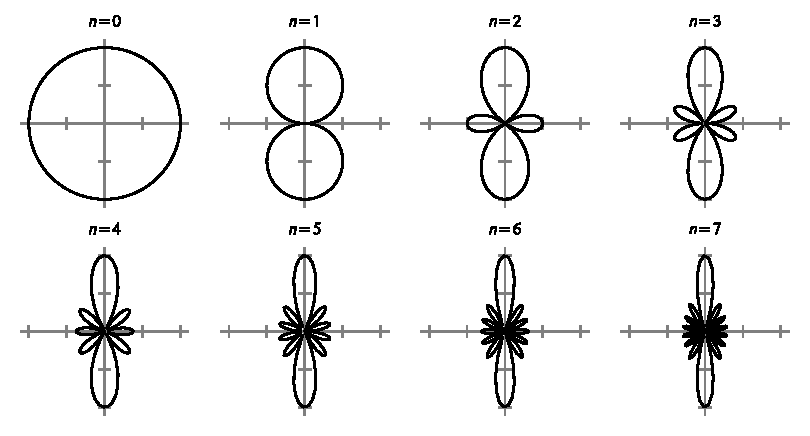
\includegraphics{legendre}

\noindent As $n$ increases, the angular scale of variations becomes finer.

The Legendre polynomials are \emph{orthogonal} in the following sense:
\begin{equation}\label{e.orthogonal}
\int_{-1}^{1}\Pl{n}(\mu)\Pl{m}(\mu)\dif \mu = \left\{
\begin{array}{lr}
	0 &  m\neq n\\
	\frac{2}{2n+1} & m=n
\end{array}\right..
\end{equation}
As a result of this orthogonality, we can decompose the radiative intensity into multipoles:
\begin{equation}\label{e.decomposition}
	I = \sum_{n=0}^{\infty} I_{n} \Pl{n}(\mu).
\end{equation}

\newthought{It is often useful to describe the intensity in terms of \newterm{moments}.} A moment is simply an angle-weighted average of the radiative intensity. For example, to take the zeroth-order moment, we multiply $I_{\nu}$ by $\mu^{0}=1$, integrate over all angles, and divide by $4\pi$. This is just the average intensity $J_{\nu} = (4\pi)^{-1}\int I_{\nu}\,\dif\Omega$. To take the first-order moment, we use a weight $\mu^{1}$:
\[
	H_{\nu} = \frac{1}{4\pi}\int_{0}^{2\pi}\int_{-1}^{1}\mu I_{\nu}\,\dif\mu\,\dif\phi.
\]
To take the second-order moment, we use a weight $\mu^{2}$:
\[
	K_{\nu} = \frac{1}{4\pi}\int_{0}^{2\pi}\int_{-1}^{1}\mu^{2} I_{\nu}\,\dif\mu\,\dif\phi.
\]
The first three moments have physically interpretable meanings: the specific radiative energy density, flux, and pressure are $U_{\nu} = (4\pi/c)J_{\nu}$, $F_{\nu} = 4\pi H_{\nu}$, and $P_{\nu} = (4\pi/c) K_{\nu}$, respectively.



Notice that we can write the weighting factors in terms of Legendre polynomials:
\begin{eqnarray*}
	J &=& \frac{1}{4\pi}\int\,\dif\phi\dif\mu\,{\color{red}\mu^{0}}\,I 
		= \frac{1}{2}\int_{-1}^{1}\dif\mu\sum_{n=0}^{\infty} \,{\color{red}\Pl{0}} I_{n} \\
	H &=& \frac{1}{4\pi}\int\,\dif\phi\dif\mu\,{\color{red}\mu^{1}}\,I 
		= \frac{1}{2}\int_{-1}^{1}\dif\mu\sum_{n=0}^{\infty} \,{\color{red}\Pl{1}} I_{n} \\
	K &=& \frac{1}{4\pi}\int\,\dif\phi\dif\mu\,{\color{red}\mu^{2}}\,I 
		= \frac{1}{2}\int_{-1}^{1}\dif\mu\sum_{n=0}^{\infty} \,{\color{red} \frac{1}{3}(2\Pl{2}+\Pl{0})} I_{n}
\end{eqnarray*}
Now we can use the orthogonality relation (eq.~[\ref{e.orthogonal}]) to compute the integrals:
\begin{eqnarray*}
	J &=& I_{0} \\
	H &=& \frac{1}{3}I_{1} \\
	K &=& \frac{1}{3}\left(\frac{2}{5}I_{2} + I_{0}\right)
		= \frac{1}{3}\left(\frac{2}{5}I_{2} + J\right)
\end{eqnarray*}
Applying the Eddington approximation, i.e., setting $K = J/3$, means that we must set $I_{2} = 0$. Once we do this, we can solve for $J$, $H$, and $K=J/3$ as functions of optical depth $\tau$. This gives us a description of the radiative intensity in terms of $J(\tau)$ and $H$,
\[
	I(\tau,\mu) = J(\tau) + 3H \Pl{1}(\mu) + \cdots \approx J(\tau) + 3H\cos\theta,
\]
which neglects the higher order terms $I_{n}\Pl{n},\forall n > 2$.
\end{sidebar}


\newcommand*{\DDtt}[1]{\frac{\dif^{2} #1}{\dif t^{2}}}
\newcommand*{\wt}{\omega t}
\newcommand*{\wot}{\omega_{0} t}
\newcommand*{\wmt}{\omega_{m} t}
\newcommand*{\womw}{(\omega_{0}^{2}-\omega^{2})}
\newcommand*{\gw}{\Gamma^{2}\omega^{2}}

\nocite{Mihalas1978Stellar-Atmosph,LeBlanc2010An-Introduction,Carroll2006An-Introduction}

\section{Atomic Lines}

Let's begin with a simple system: a mass $m$ attached to a spring with force constant $k$ as shown in Fig.~\ref{f.simple-spring}.

\begin{marginfigure}[-8\baselineskip]
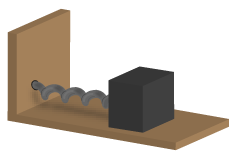
\includegraphics[width=\linewidth]{simple-spring}
\caption[A simple harmonic oscillator]{A simple harmonic oscillator: a mass $m$ on a frictionless surface attached to a  spring with force $F = -kx$.
\label{f.simple-spring}}
\end{marginfigure}

\subsection{With no driving force}

If we put the origin of our coordinate system where the mass is at rest with the spring relaxed, then the equation of motion of the mass is
\begin{equation}\label{e.SHO-basic}
	\DDtt{x} + \frac{k}{m} x = 0.
\end{equation}
You have solved this before: the most general solution is
\begin{equation}\label{e.SHO-general-solution}
	x(t) = x_{0}\cos(\wot) + \frac{v_{0}}{\omega_{0}}\sin(\wot)
\end{equation}
with $\omega_{0}^{2} = k/m$ and with $x_{0}$ and $v_{0}$ being the initial position and velocity of the mass.

\subsection{With driving at frequency $\omega \neq \omega_{0}$}

Now let's push on our mass with an oscillating force, $F\cos(\omega t)$ with $\omega\neq\omega_{0}$. A real world example would be holding a vibrating tuning fork near another fork tuned to a different frequency.  The equation of motion is now
\begin{equation}\label{e.SHO-driven}
	\DDtt{x} + \omega_{0}^{2}x = \frac{F}{m}\cos(\wt).
\end{equation}
You can verify by substitution that a general solution is
\[
	x(t) = \frac{F/m}{(\omega_{0}^{2}-\omega^{2})}\cos(\wt) + A\cos(\wot)+B\sin(\wot).
\]
Let's start with our harmonic oscillator at rest ($v_{0} = \left.\dif x/\dif t\right|_{t=0} = 0$) and at $\left. x\right|_{t=0} = 0$.  With these conditions, we can determine the constants $A$ and $B$; the solution is
\[
	x(t) = \frac{F/m}{(\omega_{0}^{2}-\omega^{2})}\left[\cos(\wt)-\cos(\wot)\right].
\]
Let's recast this by defining $\Delta = \omega_{0} - \omega$ and $\omega_{m} = (\omega_{0}+\omega)/2$.  Then
\begin{eqnarray*}
  \omega_{0}^{2}-\omega^{2} &=& (\omega_{0}-\omega)(\omega_{0}+\omega) = 2\Delta\omega_{m},\\
  \cos(\wot) &=& \cos\left(\wmt+\Delta t/2\right) = \cos(\wmt)\cos(\Delta t/2) - \sin(\wmt)\sin(\Delta t/2),\\
  \cos(\wt) &=& \cos\left(\wmt-\Delta t/2\right) = \cos(\wmt)\cos(\Delta t/2) + \sin(\wmt)\sin(\Delta t/2);
\end{eqnarray*}
and we write the solution as
\begin{equation}\label{e.beats}
	x(t) = \left[\frac{F/m}{\Delta\omega_{m}}\sin(\Delta t/2)\right]\sin(\wmt).
\end{equation}
This illustrates the phenomena of beats: the oscillation consists of a carrier signal at frequency $\omega_{m}$ with the amplitude modulated at the slower frequency $\Delta /2$.  Notice that the amplitude increases as $\Delta \to0$, i.e., $\omega\to\omega_{0}$.

\subsection{With both driving and damping}

Now let's make our model even more realistic by adding some damping.  We add a frictional force that is proportional to velocity, $F_{\mathrm{friction}} = -m\Gamma \dif x/\dif t$. Our complete equation of motion is then
\begin{equation}
	\DDtt{x} + \Gamma \DDt{x} + \omega_{0}^{2}x = \frac{F}{m}\cos(\omega t).
\end{equation}
The solution to this is straightforward to find, although the algebra is tedious (trust me on this). The general solution for initial conditions $\left.x\right|_{t=0} = x_{0}$ and $\left.\dif x/\dif t\right|_{t=0} = v_{0}$ is
\begin{eqnarray}
\label{e.general-solution-ddo}
\lefteqn{x(t) = \frac{F\womw/m}{\womw^{2}+\gw}\cos(\omega t)} && \\
	&+& \frac{\Gamma\omega F/m}{\womw^{2}+\gw}\sin(\omega t)\nonumber \\
	&+& \left[x_{0}-\frac{F\womw/m}{\womw^{2}+\gw}\right]{\color{red}e^{-\Gamma t/2}} \cos(\omega_{\Gamma}t) \nonumber\\
	&+& \left[\frac{v_{0}}{\omega_{\Gamma}}-\frac{\Gamma\omega F/m}{\womw^{2}+\gw}
	\,\frac{\omega}{\omega_{\Gamma}}\right]{\color{red}e^{-\Gamma t/2}} \sin(\omega_{\Gamma}t), 
	\nonumber
\end{eqnarray}
with
\[ 
    \omega_{\Gamma} = 
        \omega_{0}\left(1-\frac{\Gamma^{2}}{4\omega_{0}^{2}}\right)^{1/2}.
\]
Let's simplify this to the most relevant case.  First, the last two terms decay as {\color{red}$e^{-\Gamma t/2}$}: these are transients set by the initial conditions. After a time $2/\Gamma$ there will only be the first two terms, which oscillate at frequency $\omega$. 

We can simplify these first two terms even further: write
\[ \cos(\wt) = \frac{e^{i\wt}+e^{-i\wt}}{2},\quad \sin(\wt) 
    = \frac{e^{i\wt}-e^{-i\wt}}{2i}; \]
and combine terms to find
\begin{eqnarray}
    x(t) &=& \frac{F}{2m}\left[\frac{1}{\left(\omega_0^2-\omega^2\right) + i\Gamma\omega}\right]e^{i\wt} + \frac{F}{2m}\left[\frac{1}{\left(\omega_0^2-\omega^2\right) - i\Gamma\omega}\right]e^{-i\wt} \nonumber\\
    &=& \Re\left\{\frac{F}{m}\left[\frac{1}{\left(\omega_0^2-\omega^2\right) + i\Gamma\omega}\right]e^{i\wt}\right\}\label{e.oscillator-expression}
\end{eqnarray}
We use the symbol ``$\Re$'' to denote taking the real part of a complex quantity.  

From Eq.~(\ref{e.oscillator-expression}), we see that the oscillator can be described as the real part of a complex quantity $Ae^{i\wt}$, with
\[
    A = \frac{F}{m}\left[\frac{1}{\left(\omega_0^2-\omega^2\right) + i\Gamma\omega}\right].
\]
For $\omega \approx \omega_0$, we write $(\omega_0^2-\omega^2)\approx 2\omega_0(\omega_0-\omega)$ and take the square of the amplitude to find,
\begin{eqnarray}
    \left|A\right|^2 &=& \left(\frac{F}{2m\omega_0}\right)^2
        \frac{1}{(\omega_0-\omega)^2 + (\Gamma/2)^2}\nonumber\\
    &=& \frac{\pi}{2\Gamma}\left(\frac{F}{m\omega_0}\right)^2
        \left\{\frac{1}{\pi}\frac{\Gamma/2}{(\omega_0-\omega)^2 + (\Gamma/2)^2}\right\}
\end{eqnarray}
We rewrote the amplitude in the second line so that the term in $\{\cdot\}$ is normalized. The function
\[
    \mathcal{L}(\omega;\Gamma) = \frac{1}{\pi} 
        \frac{\Gamma/2}{(\omega_0-\omega)^2 + (\Gamma/2)^2}
\]
is known as a Lorentzian.  In contrast to a Gaussian, a Lorentzian is characterized by broad ``wings'' (Fig.~\ref{f.comparison}) as it goes to zero away from the central frequency $\omega_{0}$.
\begin{marginfigure}[-4\baselineskip]
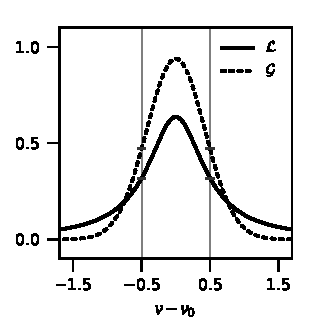
\includegraphics[width=\linewidth]{comparison}
\caption[Comparison of Lorentzian and Gaussian distributions]{\label{f.comparison}
Comparison of a Lorentzian ($\mathcal{L}$, solid line) and a Gaussian ($\mathcal{G}$, dotted line), both with $\mathrm{FWHM}=1$. The area under each curve is unity.}
\end{marginfigure}

\section{Atomic Lines}
You may be thinking, ``What does this have to do with atomic lines?'' Consider an electronic transition in an atom between two energy levels, $E_m$ and $E_n$. The natural frequency of this transition is $\nu_0 = |E_n-E_m|/h$. Light incident on the atom with frequency\sidenote{We are switching from angular frequency $\omega$ to frequency $\nu = \omega/2\pi$.} $\nu\neq\nu_0$ drives the electron at frequency $\nu$. An accelerating electron radiates, which damps the acceleration of the electron.  Classically, the transition in an atom is an electromagnetic oscillator with damping and driving terms, with cross-section\sidenote{For details, see the Box~\ref{b.line-emission}.}
\begin{equation}\label{e.semi-classical}
    \sigma = \left(\frac{\pi e^2}{m_e c}\right)
    \left\{\frac{\Gamma/4\pi}{(\nu_0-\nu)^2 + (\Gamma/4\pi)^2}\right\}.
\end{equation}
The actual value of the cross-section must be calculated using quantum mechanics. The overall shape of the cross-section is still in the form of equation~(\ref{e.semi-classical}) with opacity
\begin{equation}
    \rho\kappa_\nu = n_i \left(\frac{\pi e^2}{m_e c}\right) f_{mn}
        \left\{\frac{\Gamma/4\pi}{(\nu_0-\nu)^2 + (\Gamma/4\pi)^2}\right\}.
\end{equation}
In this equation, $f_{mn}$ is a number, called the \emph{oscillator strength}, that results from the calculation of the transition probability from state $m$ to state $n$, and $n_i$ is the density of atoms in state $m$.  The key point is that $f_{mn}$ depends only on the details of the transition: the energies, spins, and parities of the atomic states.  It does not depend on environmental parameters such as temperature and pressure.  As a result, $f_{mn}$ can be measured or computed once and then tabulated.


\begin{sidebar}[Treating line emission as a driven damped oscillator]
\label{b.line-emission}
NB. In this box, Gaussian CGS units are used for the electromagnetic field. To convert to MKS, make the following substitutions:
\begin{eqnarray*}
e &\to& \frac{1}{\sqrt{4\pi\varepsilon_0}}e\\
\bvec{E} &\to& \sqrt{4\pi\varepsilon_0}\bvec{E}\\
c &\to& (\mu_0\varepsilon_0)^{-1/2}.
\end{eqnarray*}

\newthought{Suppose we have a classical charged harmonic oscillator.}  The instantaneous power emitted by the oscillator is
\begin{equation}\label{e.larmor-power}
	 P(t) = \frac{2}{3}\frac{e^{2}}{c^{3}} |\dot{\vu}|^{2},
\end{equation}
and when averaged over a cycle is
\begin{equation}\label{e.oscillator-power}
	 \left\langle P(t) \right\rangle = \frac{e^{2}}{3c^{3}}x_{0}^{2} \omega^{4},
\end{equation}
since $\dot{\vu} = -\omega^{2}\bvec{x}_{0}\cos \omega t$. Since the oscillator is radiating, it is losing energy and is damped. Let us write the damping as $\bvec{F}_{\mathrm{rad}}\vdot \vu$; to find $\bvec{F}_{\mathrm{rad}}$, we integrate the power loss over a cycle,
\[  -\int_{t_{1}}^{t_{2}}\!\dif t\;\frac{2}{3}\frac{e^{2}}{c^{3}}\dot{\vu}\vdot\dot{\vu} 
	= -\left.\frac{2}{3}\frac{e^{2}}{c^{3}}\dot{\vu}\vdot\vu\right|_{t_{1}}^{t_{2}} 
	+ \frac{2}{3}\frac{e^{2}}{c^{3}} \int_{t_{1}}^{t_{2}}\!\dif t\;\ddot{\vu}\vdot\vu. 
\]
Since the motion is periodic, the first term vanishes and we can therefore identify 
\[ 
	\bvec{F}_{\mathrm{rad}} = \frac{2}{3}\frac{e^{2}}{c^{3}}\ddot{\vu} 
	= -m\left(\frac{2e^{2}\omega^{2}}{3c^{3}m}\right)\vu
\]
as the radiation damping term with the term in parenthesis being the damping constant $\gamma$. 
If there is an driving electric field on our oscillator, then its equation of motion becomes
\begin{equation}\label{e.eq-sho}
	m\ddot{\bvec{x}} = -m\omega_{0}^{2}\bvec{x} + e\bvec{E}e^{i\omega t} - m\gamma \dot{\bvec{x}}.
\end{equation}
Using a trial function $\bvec{x}\propto e^{i\omega t}$ gives
\[
	\bvec{x} = \frac{e}{m}\frac{E e^{i\omega t}}{(\omega_{0}^{2}-\omega^{2}) + i\omega\gamma}.
\]
Taking the second derivative w.r.t.\ time of $\bvec{x}$, substituting into eq.~(\ref{e.larmor-power}), and averaging over a cycle gives the power radiated by the oscillator,
\[
	\left\langle P(t)\right\rangle = \frac{e^{4}\omega^{4} E^{2}}{3 c^{2}m^{2}}
	\frac{1}{(\omega_{0}^{2}-\omega^{2})^{2} + \gamma^{2}\omega^{2}}.
\]
Dividing $\langle P(t)\rangle$ by the incident power per unit area, $cE^{2}/(8\pi)$, gives the cross-section:
\begin{equation}\label{e.classical-oscillator-cross-section}
	\sigma = \frac{8\pi}{3}\frac{e^{4}}{m^{2}c^{3}}
	\frac{\omega^{4}}{(\omega_{0}^{2}-\omega^{2})^{2} + \gamma^{2}\omega^{2}}.
\end{equation}
Now, for $\omega \approx \omega_{0}$, we can expand $(\omega_{0}^{2}-\omega^{2})^{2} \approx 4\omega_{0}^{2}(\omega_{0}-\omega)^{2}$; furthermore, we identify $2e^{2}\omega_{0}^{2}/(3c^{3}m) = \gamma$ and equation~(\ref{e.classical-oscillator-cross-section}) becomes
\begin{equation}\label{e.cross-section-lorentz}
	\sigma = \pi\left(\frac{e^{2}}{mc}\right)\frac{\gamma}{(\omega_{0}-\omega)^{2} + (\gamma/2)^{2}}.
\end{equation}
The line profile is Lorentzian, with a width $\gamma$. In terms of wavelength, the width is
\[ 
	\Delta \lambda = \left|\frac{\dif\lambda}{\dif\omega}\right|\gamma = \frac{2\pi c}{\omega^{2}}\gamma
	= \val{\sci{1.2}{-4}}{\textrm{\AA}}.
\]
This width is independent of the transition frequency (it is just the classical electron radius), and it is very, very small.  In a stellar atmosphere, the width is set by interactions and doppler broadening.

\newthought{To understand how impacts affect the line width}, suppose we model the oscillator as being started and stopped by impacts; in between impacts it just goes as $e^{i\omega_{0}t}$.  To get the spectrum, we take the Fourier transform,
\[
	F(\omega,t) = \int_{0}^{t}\!\dif t'\; \exp[i(\omega_{0}-\omega)t'],
\]
where $t$ is some time between impacts. Now if the impacts are distributed randomly and are uncorrelated, then the distribution of wait times follows a Poisson distribution,
\[ W(t)\,\dif t = e^{-t/\tau}\,\dif t/\tau, \]
where $\tau$ is the average time between collisions.  Using this to compute the energy spectrum, we obtain
\[ E(\omega) = \frac{1}{2\pi\tau}\int_{0}^{\infty}\!\dif t\; F(\omega,t)F^{*}(\omega,t)W(t) = \frac{1}{\pi\tau} 
	\frac{1}{(\omega_{0}-\omega)^{2} + (1/\tau)^{2}};
\]
the line profile is again Lorentzian, with a FWHM $2/\tau$.
\end{sidebar}

